\pagestyle{fancy}
\renewcommand{\theUnit}{3}
\ifthenelse{\isundefined{\UnitPageNumbers}}{}{\setcounter{page}{1}}
\rhead{Chapter \theUnit: Hypothesis Testing}
\lhead{Math 3382: Statistical Theory}
%\lhead{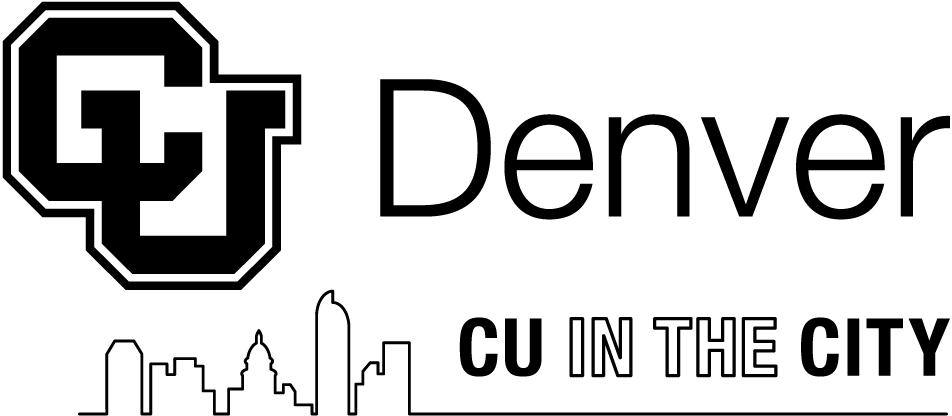
\includegraphics[width=1.25cm]{CUDenver-Logo.png}}
\rfoot{\mypage}
\cfoot{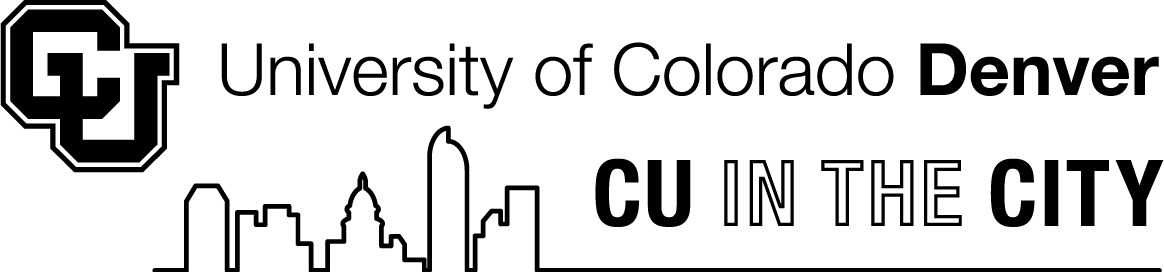
\includegraphics[width=2.25cm]{CUDenver-Logo-coverpage.png}}
\lfoot{Adam Spiegler}
\fancypagestyle{firstfooter}{\footskip = 50pt}
\renewcommand{\footrulewidth}{.4pt}
%%%%%%%%%%%%%%%%%%%%%%%%%%%
\vspace*{-20pt} \thispagestyle{firstfooter}


%\begin{tasks}[counter-format = {(tsk[a])},label-offset = {0.8em},label-format = {\color{black}\bfseries}](2)

\pagebegin{Chapter 3: Hypothesis Testing}


In \textbf{Hypothesis Testing}
\bi
\ii A claim is made about the population, and researchers want to determine which of the two competing claims is more likely.
\ii Researchers collect data and compare statistics.
\ii Based on data collected, researchers assess which of the claims seems more likely.
\ei

Some examples of questions that could be answered using a hypothesis test are:
\bi
\ii What is a better method to help smokers quit:  give them money for successfully quitting, or penalize them if they don’t stop?
\ii What is the better mailer to send in order to nudge voters into actually voting?
\ii What is a more effective government assistance program, giving people food stamps or cash?
\ei

\bbox
We refer to the two competing hypotheses as the \textbf{\colorb{null hypothesis}}, denoted by \colorb{$H_0$}, and the \colorr{\textbf{alternative hypothesis}}, denoted by \colorr{$H_a$}.
\bi
\ii \colorb{$H_0$ is the boring claim that nothing interesting is happening.}
\ii \colorr{$H_a$ is new or different result a researcher is trying to establish or find evidence for.}
\ei

\textbf{Collect sample data. Then assess the competing claims.} 
\ebox


\bb
\ii Telepathy is the ability of an individual to communicate thoughts and ideas by means other than the known senses. I claim that I do have telepathy. There are two possibilities: either I do or I do not. Which claim is the null hypothesis and which is the alternative?  \vfill


\ii There are many experiments we could try to run to test these competing claims. For example, I will think of a letter A, B, C, or D and communicate this letter to each of you. If I could collect data from everyone in the population, and let $p$ denote the proportion of all people that say the letter I was thinking of. If $H_0$ is true, what would you expect the value of $p$ to be? If $H_a$ is true, what would you expect the value of $p$ to be?  \vfill


\ii There are (about) 25 people in this room. If $\hat{p}$ denotes the proportion of the people in this class that say the letter I was
thinking of. What would be enough evidence to convince you that I do have telepathy? What would need to be true about $\hat{p}$?
 \vfill
 
\ee

\clearpage

\pagebegin{Section 3.2: Hypotheses and Significance}

\bbox
The general steps for a hypothesis test are summarized below.
\bi
\ii Set the hypotheses in terms of population parameters. \colorb{Use an equal sign in the null hypothesis}. Depending on what researchers are hoping to prove \colorr{use $\ne$, $<$, or $>$ in the alternative hypothesis}.
\ii Collect data and define a statistic that can be used to assess the hypotheses. Compute the \textbf{test statistic} using the collected data.
\ii Assume $H_0$ is true. Under this assumption, is the observed test statistic likely? Unlikely?
If the \textbf{\colorb{test statistic is very unlikely}} (under the assumption in $H_0$):
\bi
\ii[$\circ$] The test is \textbf{\colorb{statistically significant}}.
\ii[$\circ$] We have convincing evidence the null hypothesis is wrong.
\ii[$\circ$] \textbf{\colorb{We reject $\mathbf{H_0}$ and accept the alternative hypothesis}}.
\ei
\ii If the \textbf{\colorr{test statistic seems plausible}} (under the assumption in $H_0$):
\bi
\ii[$\circ$] The test is \textbf{\colorr{not statistically significant}}.
\ii[$\circ$] We cannot be sure whether the claim in $H_0$ is true or not.
\ii[$\circ$] The \textbf{\colorr{test is inconclusive}}. We neither reject nor accept $H_0$.
\ei
%\ii How unlikely does the test statistic need to be in order to be significant?
\ei
\ebox


\bb[resume]
\ii A 2004 article\footnote{\href{http://rady.ucsd.edu/faculty/directory/gneezy/pub/docs/splitting-bill.pdf}{\underline{http://rady.ucsd.edu/faculty/directory/gneezy/pub/docs/splitting-bill.pdf}}} from the Economic Journal studied the so called unscrupulous diner’s dilemma.  

\begin{quote}
The unscrupulous diner’s dilemma is a problem faced frequently in social settings. When a group of diners jointly enjoys a meal at a restaurant, often an unspoken agreement exists to divide the check equally. A selfish diner could thereby enjoy exceptional dinners at bargain prices…This dilemma typifies a class of serious social problems\footnote{\href{http://www.uvm.edu/~pdodds/files/papers/others/1994/glance1994a.pdf}{\underline{http://www.uvm.edu/~pdodds/files/papers/others/1994/glance1994a.pdf}}} from environmental protection and resource conservation to eliciting charity donations and slowing arms races.
\end{quote}

Researchers wanted to test whether people order more food and beverages when they know the bill is going to split evenly, or do they order the same amount regardless of whether they are splitting the bill or paying individually.
\bb
\ii State the null and alternative hypotheses in words.  \vfill

\clearpage

\ii To test the claims, participants were randomly assigned into two tables, each with four people. One table (even-split group) was randomly picked and told they were going to evenly-split the bill. The other table (control) was told each person was going to pay for what they ordered. The mean amount ordered by the control group was $\$8.67$. Which of following samples for the even-split group is the most statistically significant? Support your answer with an explanation.

\begin{tasks}[counter-format = {(tsk[r])},label-offset = {0.8em},label-format = {\color{black}\bfseries}](4)
\task $\$4.67$
\task $\$8.50$
\task $\$8.80$
\task $\$11.23$
\end{tasks}

 \vfill

\ii Restate the hypotheses in terms of the parameters $\mu_{\rm{even}}$ and $\mu_{\rm{control}}$, the true mean amount ordered by people that evenly-split and invidiually pay for the bill, respectively.

 \vfill

\ii If the table below gives the amounts ordered by each of the four people in each group, what is the value of the test statistic?

\begin{center}
\begin{tabular}{|cccc|}
\hline
\multicolumn{4}{c}{Even-Split}\\
\hline
$\$15.00$ & $\$8.00$ & $\$8.75$ & $\$13.17$\\
\hline
\end{tabular}
\ \ \ \ \ \ \ \ \ \ \ \ \ \ \ \ \ \ \ \ \ \ \ \ \
\begin{tabular}{|cccc|}
\hline
\multicolumn{4}{c}{Control}\\
\hline
$\$8.50$ & $\$7.90$ & $\$10.85$ & $\$7.43$\\
\hline
\end{tabular}
\end{center}

 \vfill

\ii Based on the test statistic, what do you think we can conclude about the two competing claims?
 \vfill
\ee
\ee

\clearpage

\pagebegin{Example: Social Pressure and Voter Turnout}

\bb[resume]
\ii A 2008 experiment\footnote{\href{http://isps.yale.edu/sites/default/files/publication/2012/12/ISPS08-001.pdf}{\underline{http://isps.yale.edu/sites/default/files/publication/2012/12/ISPS08-001.pdf}}}
at Yale aimed to determine whether positive or negative pressure is more effective at improving voter turnout.

\begin{quote}
Voter turnout theories based on rational self-interested behavior generally fail to predict significant turnout unless they account for the utility that citizens receive from performing their civic duty. We distinguish between two aspects of this type of utility, 
\end{quote}

\begin{multicols}{2}
One group received a mailing emphasizing the intrinsic (internal) satisfaction for voting:

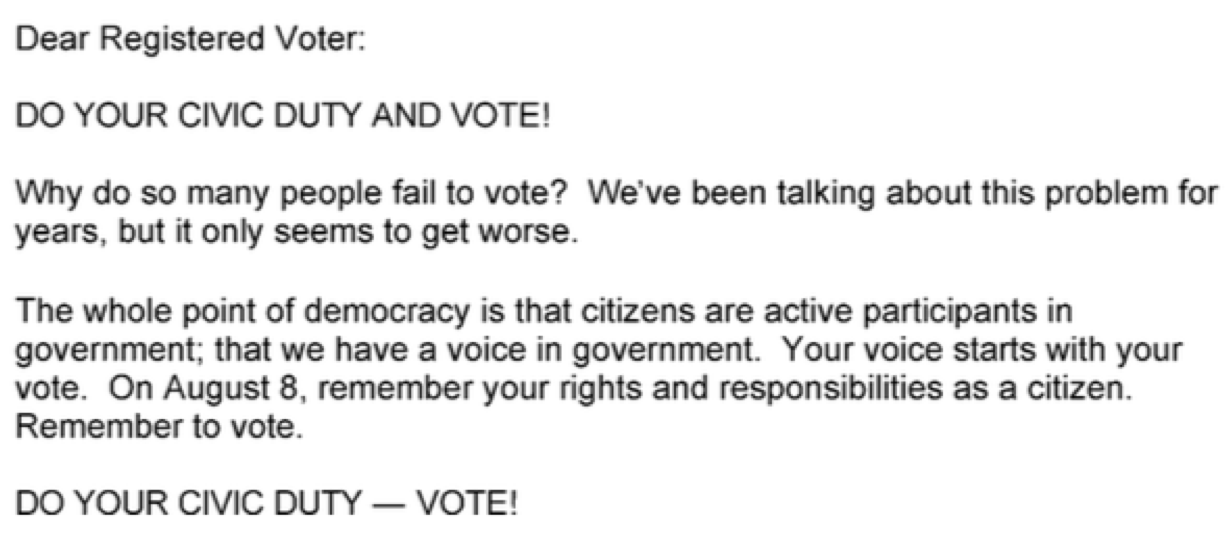
\includegraphics[width=0.48\tw]{18/fig-intrinsic.png}


\columnbreak

Another group received a mailing placing extrinsic (outside) pressure on people to vote:

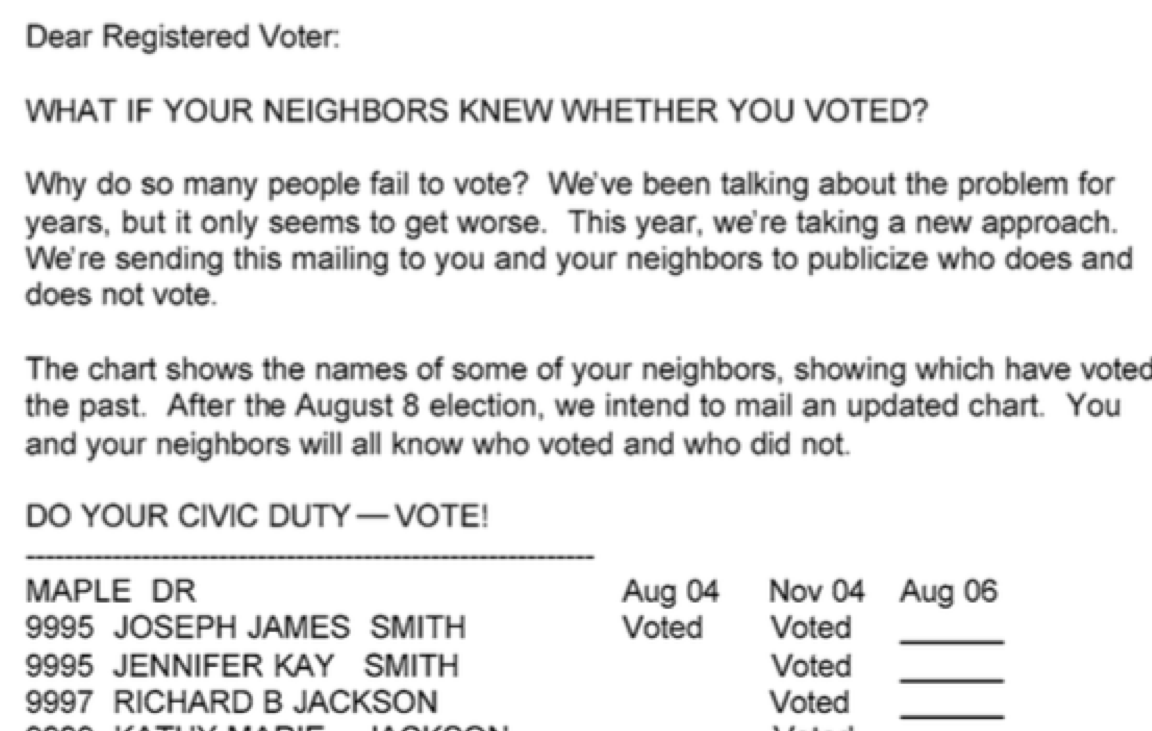
\includegraphics[width=0.48\tw]{18/fig-extrinsic.png}

\end{multicols}

\bb
\ii State the null and alternative hypotheses in words the researches can use to test whether positive or negative pressure is more effective at improving voter turnout.
\vfill
\ii What is a possible test statistic the researchers could use to assess the competing claims in your previous answer?
\vfill

\ii Using the test statistic in your previous answer, restate your null and alternative hypotheses using appropriate notation.
\vfill
\ee 
\ee

\clearpage

\pagebegin{Calculating $P$-Values}

\bbox
\bi
\ii The \textbf{$\mathbf{P}$-value} is the probability that you would get a random sample with a test statistic as or more extreme
as the observed test statistic if the null hypothesis were true.
\ii The \colorb{smaller the $P$-value} is, the \colorb{less likely the sample} is, and there is evidence that \colorb{contradicts $H_0$} and \colorb{supports $H_a$}.
\ii \textbf{\colorb{Thus, the smaller the $P$-value, the more statistically significant the result is.}}
\ei
\ebox

\bb[resume]
\ii In the telepathy example, let $T$ be the number of people out of 25 that say the letter I was thinking.  If we observed that 20 out of 25 people say the letter I was thinking.
\bb
\ii Calculate the $P$-value of the observed test statistic. In other words, in 25 identical and independent trials each with likelihood of success $p = 0.25$, compute $P(T \geq 20)$.

\vfill

\ii Based on the value of the $P$-value, what can we conclude about my telepathy ability?

\vspace{1.25in}

\ee
\ee

\bbox
The \textbf{\colorb{null distribution}} is the distribution of the test statistic \colorb{if the null hypothesis is true}.
\ebox

\bb[resume]
\ii What is the null distribution for the previous telepathy example?
\vspace{1.25in}
\ee

